%%
%% This is file `sample-acmtog.tex',
%% generated with the docstrip utility.
%%
%% The original source files were:
%%
%% samples.dtx  (with options: `all,journal,bibtex,acmtog')
%% 
%% IMPORTANT NOTICE:
%% 
%% For the copyright see the source file.
%% 
%% Any modified versions of this file must be renamed
%% with new filenames distinct from sample-acmtog.tex.
%% 
%% For distribution of the original source see the terms
%% for copying and modification in the file samples.dtx.
%% 
%% This generated file may be distributed as long as the
%% original source files, as listed above, are part of the
%% same distribution. (The sources need not necessarily be
%% in the same archive or directory.)
%%
%%
%% Commands for TeXCount
%TC:macro \cite [option:text,text]
%TC:macro \citep [option:text,text]
%TC:macro \citet [option:text,text]
%TC:envir table 0 1
%TC:envir table* 0 1
%TC:envir tabular [ignore] word
%TC:envir displaymath 0 word
%TC:envir math 0 word
%TC:envir comment 0 0
%%
%% The first command in your LaTeX source must be the \documentclass
%% command.
%%
%% For submission and review of your manuscript please change the
%% command to \documentclass[manuscript, screen, review]{acmart}.
%%
%% When submitting camera ready or to TAPS, please change the command
%% to \documentclass[sigconf]{acmart} or whichever template is required
%% for your publication.
%%
%%

\documentclass[sigconf,nonacm]{acmart}

%%
%% \BibTeX command to typeset BibTeX logo in the docs
\AtBeginDocument{%
  \providecommand\BibTeX{{%
    Bib\TeX}}}

%% Rights management information.  This information is sent to you
%% when you complete the rights form.  These commands have SAMPLE
%% values in them; it is your responsibility as an author to replace
%% the commands and values with those provided to you when you
%% complete the rights form.
\setcopyright{acmlicensed}
\copyrightyear{2018}
\acmYear{2018}
\acmDOI{XXXXXXX.XXXXXXX}

%%
%% These commands are for a JOURNAL article.
\acmJournal{TOG}
\acmVolume{37}
\acmNumber{4}
\acmArticle{111}
\acmMonth{8}

%%
%% Submission ID.
%% Use this when submitting an article to a sponsored event. You'll
%% receive a unique submission ID from the organizers
%% of the event, and this ID should be used as the parameter to this command.
%%\acmSubmissionID{123-A56-BU3}

%%
%% For managing citations, it is recommended to use bibliography
%% files in BibTeX format.
%%
%% You can then either use BibTeX with the ACM-Reference-Format style,
%% or BibLaTeX with the acmnumeric or acmauthoryear sytles, that include
%% support for advanced citation of software artefact from the
%% biblatex-software package, also separately available on CTAN.
%%
%% Look at the sample-*-biblatex.tex files for templates showcasing
%% the biblatex styles.
%%

%%
%% The majority of ACM publications use numbered citations and
%% references.  The command \citestyle{authoryear} switches to the
%% "author year" style.
%%
%% If you are preparing content for an event
%% sponsored by ACM SIGGRAPH, you must use the "author year" style of
%% citations and references.
\citestyle{acmauthoryear}

\usepackage{anyfontsize}
\usepackage{listings}
\usepackage[nolist]{acronym}
% These packages are required for list code snippets.
\usepackage{xcolor}
\usepackage{color}
% The following special color definitions are used in the IST Thesis
\definecolor{forestgreen}{RGB}{34,139,34}
\definecolor{orangered}{RGB}{239,134,64}
\definecolor{lightred}{rgb}{1,0.4,0.5}
\definecolor{orange}{rgb}{1,0.45,0.13}
\definecolor{darkblue}{rgb}{0.0,0.0,0.6}
\definecolor{lightblue}{rgb}{0.1,0.57,0.7}
\definecolor{gray}{rgb}{0.4,0.4,0.4}
\definecolor{lightgray}{rgb}{0.95, 0.95, 0.95}
\definecolor{darkgray}{rgb}{0.4, 0.4, 0.4}
\definecolor{editorGray}{rgb}{0.95, 0.95, 0.95}
\definecolor{editorOcher}{rgb}{1, 0.5, 0} % #FF7F00 -> rgb(239, 169, 0)
\definecolor{chaptergrey}{rgb}{0.6,0.6,0.6}
\definecolor{editorGreen}{rgb}{0, 0.5, 0} % #007C00 -> rgb(0, 124, 0)
\definecolor{olive}{rgb}{0.17,0.59,0.20}
\definecolor{brown}{rgb}{0.69,0.31,0.31}
\definecolor{purple}{rgb}{0.38,0.18,0.81}

\newcommand{\changed}[1]{\textcolor{orange}{#1}}

% Symbols for linear logic
\usepackage{cmll}

% For proof trees
\usepackage{bussproofs}

% For multiply counters, which I use for indentation in class environments
\usepackage{calc}

% These are useful!
\providecommand\todo{}
\renewcommand{\todo}[1]{\textcolor{red}{\textbf{#1}}}

% Useful for CLASS snippets
\lstdefinelanguage{CLASS}{
    morekeywords={proc, cut, close, wait, case, of, send, recv, choice, offer, !, ?, print, println, par, let, share, put, take, cell},
    morekeywords=[2]{lint, colint, lbool, colbool, state, usage},
    sensitive=true,
    moredelim=[is][keywordstyle2]{@}{@},
}

% Useful for IR snippets
\lstdefinelanguage{IR}{
    morekeywords={int, bool, string, tag, cont, exponential, cell, type, isValue},
    morecomment=[l]{//},
    sensitive=true,
}

% Color BNF with strings
\lstdefinelanguage{BNF}{
    morekeywords={nl, pid, lab, int, loc, t, t1, t2, c, c1, c2, d, d1, d2, e, prog, proc, entry, block, instr, sl, st, sc, ofs, locb, reqs, flag, expr, tflg, targ, carg, darg, parg, pargs, earg, eargs, case, if, else, str, bool, src, dst},
    sensitive=true,
    morestring=[b]",
    morestring=[b]',
    morecomment=[l]{//},
    morecomment=[s]{/*}{*/},
    moredelim=[is][keywordstyle2]{@}{@},
    alsoletter={:},
    morekeywords=[2]{::=,|,*,+,?},
}

% Slot names
\newcommand{\irs}[1]{\text{\textcolor{lightblue}{#1}}}
\newcommand{\ints}{\irs{int}}
\newcommand{\bools}{\irs{bool}}
\newcommand{\strings}{\irs{string}}
\newcommand{\tags}{\irs{tag}}
\newcommand{\conts}{\irs{cont}}
\newcommand{\exponentials}{\irs{exponential}}
\newcommand{\types}{\irs{type}}
\newcommand{\cells}[1]{\irs{cell}\left[#1\right]}
\newcommand{\vars}[1]{t_{#1}}

% Slot trees
\newcommand{\nilst}{\left[\right]}
\newcommand{\seqst}[1]{\left[#1\right]}
\newcommand{\tagst}[1]{\irs{tag}\left[#1\right]}
\newcommand{\flagsst}[3]{\irs{flags}\left<#1\right>\left[#2\tagsepst{}#3\right]}
\newcommand{\combst}[1]{\text{$<$}#1\text{$>$}}
\newcommand{\tagsepst}{\text{ | }}
\newcommand{\concatst}[2]{#1\oplus#2}

% Slot offset and data location
\newcommand{\offs}[2]{#1\text{$\sim$}#2}
\newcommand{\dataol}[2]{#1.#2}
\newcommand{\datal}[3]{\dataol{#1}{\offs{#2}{#3}}}

% Some notation commands
\newcommand{\sizeof}[1]{\phi\bigl(#1\bigr)}
\newcommand{\dual}[1]{\overline{#1}}
\newcommand{\getinstructions}[3]{\mathcal{I}_P(#1,\,#2,\,#3)}
\newcommand{\getendpoints}[2]{\mathcal{E}(#1,\,#2)}
\newcommand{\getexpression}[2]{\mathcal{I}_E(#1,\,#2)}
\newcommand{\makeblock}[1]{#1 \leftarrow \text{new}_{\text{b}}()}
\newcommand{\makecont}[1]{#1 \leftarrow \text{new}_{\text{c}}()}
\newcommand{\makedata}[2]{#1 \leftarrow \text{new}_{\text{d}}(#2)}
\newcommand{\makedrop}[3]{#1 \leftarrow \text{new}_{\text{e}}(#2,\,#3)}

% Type names
\newcommand{\classt}[1]{\textbf{\textcolor{forestgreen}{#1}}}
\newcommand{\closet}{\classt{close}}
\newcommand{\waitt}{\classt{wait}}
\newcommand{\lintt}{\classt{lint}}
\newcommand{\colintt}{\classt{colint}}
\newcommand{\lboolt}{\classt{lbool}}
\newcommand{\colboolt}{\classt{colbool}}
\newcommand{\lstringt}{\classt{lstring}}
\newcommand{\colstringt}{\classt{colstring}}
\newcommand{\choicet}[1]{\classt{choice of}\,\{#1\}}
\newcommand{\offert}[1]{\classt{offer of}\,\{#1\}}
\newcommand{\labelt}[2]{\classt{$|$\##1}:#2}
\newcommand{\sendt}[2]{\classt{send}\,#1;#2}
\newcommand{\recvt}[2]{\classt{recv}\,#1;#2}
\newcommand{\bangt}[1]{\classt{!}#1}
\newcommand{\whynott}[1]{\classt{?}#1}
\newcommand{\sendtyt}[2]{\classt{sendty}\,#1;#2}
\newcommand{\recvtyt}[2]{\classt{recvty}\,#1;#2}
\newcommand{\statet}[1]{\classt{state}\,#1}
\newcommand{\statelt}[1]{\classt{statel}\,#1}
\newcommand{\usaget}[1]{\classt{usage}\,#1}
\newcommand{\usagelt}[1]{\classt{usagel}\,#1}
\newcommand{\affinet}[1]{\classt{affine}\,#1}
\newcommand{\coaffinet}[1]{\classt{coaffine}\,#1}
\newcommand{\dualt}[1]{\classt{$\sim$}#1}
\newcommand{\rect}[2]{\classt{rec}\ #1;\,#2}
\newcommand{\corect}[2]{\classt{corec}\ #1;\,#2}

% Process names
\newcommand{\classp}[1]{\textbf{\textcolor{darkblue}{#1}}}
\newcommand{\emptyp}{\classp{()}}
\newcommand{\fwdp}{\classp{fwd}}
\newcommand{\cutp}{\classp{cut}}
\newcommand{\parp}{\classp{par}}
\newcommand{\closep}{\classp{close}}
\newcommand{\waitp}{\classp{wait}}
\newcommand{\casep}{\classp{case of}}
\newcommand{\labelp}[1]{\classp{\##1}}
\newcommand{\sendp}{\classp{send}}
\newcommand{\recvp}{\classp{recv}}
\newcommand{\bangp}{\classp{!}}
\newcommand{\whynotp}{\classp{?}}
\newcommand{\callp}{\classp{call}}
\newcommand{\sendtyp}{\classp{sendty}}
\newcommand{\recvtyp}{\classp{recvty}}
\newcommand{\unfoldmup}{\classp{unfold$_\mu$}}
\newcommand{\unfoldnup}{\classp{unfold$_\nu$}}
\newcommand{\corecp}{\classp{corec}}
\newcommand{\sharep}{\classp{share}}
\newcommand{\affinep}{\classp{affine}}
\newcommand{\discardp}{\classp{discard}}
\newcommand{\usep}{\classp{use}}
\newcommand{\cellp}{\classp{cell}}
\newcommand{\releasep}{\classp{release}}
\newcommand{\takep}{\classp{take}}
\newcommand{\putp}{\classp{put}}
\newcommand{\ifp}{\classp{if}}
\newcommand{\elsep}{\classp{else}}
\newcommand{\letp}{\classp{let}}
\newcommand{\scanp}{\classp{scan}}
\newcommand{\printp}{\classp{print}}
\newcommand{\printlnp}{\classp{println}}

% CLASS
\newcommand{\fwdc}[2]{\fwdp\,#1\,#2}
\newcommand{\cutc}[3]{\cutp\,\{#1\,\classp{$|$}#2\classp{$|$}\,#3\}}
\newcommand{\parc}[2]{\parp\,\{#1\,\classp{$||$}\,#2\}}
\newcommand{\emptyc}{\emptyp}
\newcommand{\closec}[1]{\closep\,#1}
\newcommand{\waitc}[1]{\waitp\,#1;}
\newcommand{\choosec}[2]{\classp{\##1}\ #2;}
\newcommand{\casec}[2]{\classp{case}\,#1\,\classp{of}\,\{#2\}}
\newcommand{\labelc}[2]{\classp{$|$}\labelp{#1}:#2}
\newcommand{\sendc}[3]{\sendp\,#1(#2.\,#3);}
\newcommand{\recvc}[2]{\recvp\,#1(#2);}
\newcommand{\bangc}[2]{\bangp\,#1(#2);}
\newcommand{\whynotc}[1]{\whynotp\,#1;}
\newcommand{\callc}[2]{\callp\,#1(#2);}
\newcommand{\sendtyc}[2]{\sendtyp\,#1(#2);}
\newcommand{\recvtyc}[2]{\recvtyp\,#1(#2);}
\newcommand{\unfoldmuc}[1]{\unfoldmup\,#1;}
\newcommand{\unfoldnuc}[1]{\unfoldnup\,#1;}
\newcommand{\corecc}[4]{\corecp\,#1(#2);\,#3\ [#4]}
\newcommand{\typedefc}[2]{\classp{type}\ #1\,\{#2\};;}
\newcommand{\rectypedefc}[2]{\classp{rec}\ \typedefc{#1}{#2}}
\newcommand{\typedefgc}[3]{\classp{type}\ #1(#2)\,\{#3\};;}
\newcommand{\rectypedefgc}[3]{\classp{rec}\ \typedefgc{#1}{#2}{#3}}
\newcommand{\procdefc}[3]{\classp{proc}\ \texttt{#1}(#2)\,\{#3\};;}
\newcommand{\procdefgc}[4]{\classp{proc}\ \texttt{#1}\langle#2\rangle(#3)\,\{#4\};;}
\newcommand{\recprocdefc}[3]{\classp{rec}\ \procdefc{#1}{#2}{#3}}
\newcommand{\recprocdefgc}[4]{\classp{rec}\ \procdefgc{#1}{#2}{#3}{#4}}
\newcommand{\proccallc}[2]{\texttt{#1}(#2)}
\newcommand{\proccallgc}[3]{\texttt{#1}\langle#2\rangle(#3)}
\newcommand{\sharec}[3]{\sharep\,#1\,\{#2\,\classp{$||$}\,#3\}}
\newcommand{\affinec}[1]{\affinep\,#1;}
\newcommand{\discardc}[1]{\discardp\,#1}
\newcommand{\usec}[1]{\usep\,#1;}
\newcommand{\cellc}[3]{\cellp\,#1(#2.\,#3)}
\newcommand{\cellfc}[2]{\cellp\,#1(#2)}
\newcommand{\releasec}[1]{\releasep\,#1}
\newcommand{\takec}[2]{\takep\,#1(#2);}
\newcommand{\putc}[3]{\putp\,#1(#2.\,#3);}
\newcommand{\putfc}[2]{\putp\,#1(#2);}
\newcommand{\ifc}[3]{\ifp\,#1\,\{#2\}\,\elsep\,\{#3\}}
\newcommand{\letc}[2]{\letp\,#1\,#2}
\newcommand{\scanc}[1]{\scanp(#1)}
\newcommand{\printc}[1]{\printp(#1);}
\newcommand{\printlnc}[1]{\printlnp(#1);}

% IR Data Locations
\newcommand{\slotoffset}[2]{#1\text{$\sim$}#2}
\newcommand{\offsetpast}[1]{\text{past}(#1)}
\newcommand{\offsetfuture}[1]{\text{future}(#1)}

% CLASS definitions
\newcommand{\slots}[2]{\mathcal{S}(#1,\,#2)}
\newcommand{\allslots}[2]{\mathcal{S}_T(#1,\,#2)}
\newcommand{\alllocalslots}[2]{\mathcal{S}_L(#1,\,#2)}

% Compiler environment accessors
\newcommand{\polarityof}[2]{#1_{p}(#2)}
\newcommand{\typeidof}[2]{#1_{t}(#2)}
\newcommand{\continuationof}[2]{#1_c(#2)}
\newcommand{\localdataof}[2]{#1_d(#2)}
\newcommand{\offsetof}[2]{#1_o(#2)}
\newcommand{\readlocof}[2]{#1_r(#2)}
\newcommand{\writelocof}[2]{#1_w(#2)}
\newcommand{\advancech}[6]{#1[#2 \overset{#3,#4}{\oplus} (#5,\,#6)]}

% C generator notation
\newcommand{\arch}{\mathcal{T}}
\newcommand{\archlayout}[1]{\arch(\texttt{#1})}
\newcommand{\slotlayout}[2]{\mathcal{L}_{\arch}(#1,\,#2)}
\newcommand{\layoutofvar}[2]{#1(#2)}
\newcommand{\envlayout}{\mathcal{E}}
\newcommand{\envlayouteps}[1]{\envlayout_\text{eps}(#1)}
\newcommand{\envlayoutdrop}[1]{\envlayout_\text{e}(#1)}
\newcommand{\envlayouttype}[2]{\envlayout_\text{ty}(#1, #2)}
\newcommand{\envlayoutcont}[2]{\envlayout_\text{c}(#1, #2)}
\newcommand{\envlayoutlocal}[2]{\envlayout_\text{d}(#1, #2)}

% Optimizer notation
\newcommand{\typeenv}{\theta}
\newcommand{\isvalue}[1]{\mathcal{V}_\typeenv(#1)}
\newcommand{\isdroppable}[1]{\mathcal{D}_\typeenv(#1)}
\newcommand{\iscloneable}[1]{\mathcal{C}_\typeenv(#1)}
\newcommand{\impossible}{\mathbf{impossible}}
\newcommand{\guaranteed}{\mathbf{guaranteed}}
\newcommand{\dependent}[1]{\mathbf{dependent}(#1)}
\newcommand{\depisvalue}[1]{\mathcal{V}(#1)}
\newcommand{\depisdroppable}[1]{\mathcal{D}(#1)}
\newcommand{\depiscloneable}[1]{\mathcal{C}(#1)}

% Session modes
\newcommand{\writemode}{\texttt{write}}
\newcommand{\readmode}{\texttt{read}}

% Indented CLASS environment
\newcounter{indentlevel}
\newlength{\indentstep}
\newenvironment{class}
{
    \begingroup

    \setcounter{indentlevel}{0}

    \setlength{\indentstep}{1.5em}

    \newcommand{\iz}{\addtocounter{indentlevel}{1}}
    \newcommand{\dz}{\addtocounter{indentlevel}{-1}}
    \newcommand{\pz}{\hspace*{\the\indentstep*\value{indentlevel}}}
    \newcommand{\z}{\\&\pz}

    % CLASS
    \let\cuti\cutc
    \renewcommand{\cutc}[3]{\cuti{\iz\z##1\z}{##2}{\z##3\dz\z}}
    \let\pari\parc
    \renewcommand{\parc}[2]{\pari{\iz\z##1\z}{\z##2\dz\z}}
    \let\waiti\waitc
    \renewcommand{\waitc}[1]{\waiti{##1}\z}
    \let\sendi\sendc
    \renewcommand{\sendc}[3]{\sendi{##1}{##2}{##3}\z}
    \let\recvi\recvc
    \renewcommand{\recvc}[2]{\recvi{##1}{##2}\z}
    \let\choosei\choosec
    \renewcommand{\choosec}[2]{\choosei{##1}{##2}\z}
    \let\casei\casec
    \renewcommand{\casec}[2]{\casei{##1}{##2\z}}
    \let\labeli\labelc
    \renewcommand{\labelc}[2]{\iz\z\labeli{##1}{##2}\dz}
    \let\unfoldmui\unfoldmuc
    \renewcommand{\unfoldmuc}[1]{\unfoldmui{##1}\z}
    \let\unfoldnui\unfoldnuc
    \renewcommand{\unfoldnuc}[1]{\unfoldnui{##1}\z}
    \let\procdefi\procdefc
    \renewcommand{\procdefc}[3]{\procdefi{##1}{##2}{\iz\z##3\dz\z}}
    \let\procdefgi\procdefgc
    \renewcommand{\procdefgc}[4]{\procdefgi{##1}{##2}{##3}{\iz\z##4\dz\z}}
    \let\typedefi\typedefc
    \renewcommand{\typedefc}[2]{\typedefi{##1}{\iz\z##2\dz\z}}
    \let\typedefgi\typedefgc
    \renewcommand{\typedefgc}[3]{\typedefgi{##1}{##2}{\iz\z##3\dz\z}}
    \let\printi\printc
    \renewcommand{\printc}[1]{\printi{##1}\z}
    \let\printlni\printlnc
    \renewcommand{\printlnc}[1]{\printlni{##1}\z}
    \let\affinei\affinec
    \renewcommand{\affinec}[1]{\affinei{##1}\z}
    \let\usei\usec
    \renewcommand{\usec}[1]{\usei{##1}\z}
    \let\discardi\discardc
    \renewcommand{\discardc}[1]{\discardi{##1}}
    \let\celli\cellc
    \renewcommand{\cellc}[3]{\celli{##1}{##2}{\iz\z##3\dz\z}}
    \let\cellfi\cellfc
    \renewcommand{\cellfc}[2]{\cellfi{##1}{##2}\z}
    \let\takei\takec
    \renewcommand{\takec}[2]{\takei{##1}{##2}\z}
    \let\puti\putc
    \renewcommand{\putc}[3]{\puti{##1}{##2}{##3}\z}
    \let\putfi\putfc
    \renewcommand{\putfc}[2]{\putfi{##1}{##2}\z}
    \let\sharei\sharec
    \renewcommand{\sharec}[3]{\sharei{##1}{\iz\z##2\z}{\z##3\dz\z}}

    $$
        \begin{aligned}
             & \pz
            }
            {
        \end{aligned}
    $$

    \endgroup
}

% Compilation environment
\newenvironment{compilation}[4]
{
    \begingroup
    % IR
    \newcommand{\beginir}{\\&\hspace{2.5em}}
    \newcommand{\mkzeroargir}[2]{\newcommand{##1}{\beginir\texttt{##2}()}}
    \newcommand{\mkoneargir}[2]{\newcommand{##1}[1]{\beginir\texttt{##2}(####1)}}
    \newcommand{\mktwoargir}[2]{\newcommand{##1}[2]{\beginir\texttt{##2}(####1, ####2)}}
    \newcommand{\mkthreeargir}[2]{\newcommand{##1}[3]{\beginir\texttt{##2}(####1, ####2, ####3)}}
    \newcommand{\mkfourargir}[2]{\newcommand{##1}[4]{\beginir\texttt{##2}(####1, ####2, ####3, ####4)}}
    \newcommand{\labelir}[1]{\\&\hspace{1.25em}\texttt{##1:}}
    \renewcommand{\comment}[1]{\quad\textcolor{forestgreen}{\%\ ##1}}
    \newcommand{\commentline}[1]{\beginir\textcolor{forestgreen}{\%\ ##1}}

    \mkoneargir{\launchthread}{launchThread}
    \mkoneargir{\pushtask}{pushTask}
    \mkoneargir{\poptask}{popTask}
    \mktwoargir{\finishcont}{finish}
    \mkoneargir{\continue}{continue}
    \mkthreeargir{\bindcontinuation}{bindContinuation}
    \mkthreeargir{\forward}{forward}
    \mktwoargir{\branchtag}{branchTag}
    \mktwoargir{\branchflags}{branchFlags}
    \mktwoargir{\writetype}{writeType}
    \mktwoargir{\writetag}{writeTag}
    \mktwoargir{\writeexpr}{writeExpression}
    \mktwoargir{\writescan}{writeScan}
    \mktwoargir{\writecell}{writeCell}
    \mkthreeargir{\writeexp}{writeExponential}
    \mktwoargir{\writecontinuation}{writeContinuation}
    \mkoneargir{\lockcell}{lockCell}
    \mkoneargir{\unlockcell}{unlockCell}
    \mkoneargir{\acquirecell}{acquireCell}
    \mkoneargir{\releasecell}{releaseCell}
    \mkoneargir{\print}{print}
    \mkoneargir{\printline}{printLine}
    \mkfourargir{\continueifneg}{continueIfNegative}
    \mkthreeargir{\moveslots}{moveSlots}
    \mkthreeargir{\cloneslots}{cloneSlots}
    \mktwoargir{\dropslots}{dropSlots}
    \mkthreeargir{\callprocess}{callProcess}
    \mkoneargir{\deferdrop}{deferDrop}

    \mkoneargir{\newtask}{newTask}
    \mkzeroargir{\nexttask}{nextTask}
    \mkthreeargir{\initcontinuation}{initializeContinuation}
    \mkoneargir{\freesession}{freeSession}
    \mkthreeargir{\call}{call}
    \mkoneargir{\flip}{flip}
    \mktwoargir{\fwd}{fwd}
    \mkoneargir{\pushclose}{pushClose}
    \mkoneargir{\popclose}{popClose}
    \mktwoargir{\pushtag}{pushTag}
    \mktwoargir{\poptag}{popTag}
    \mktwoargir{\pushsession}{pushSession}
    \mktwoargir{\popsession}{popSession}
    \newcommand{\hasexitpoint}{\texttt{exit point}}
    \newcommand{\recurse}[3]{\beginir\getinstructions{##1}{##2}{##3}}

    $$
        \begin{aligned}
             & \getendpoints{#1}{#3} \equiv #4 \\
             & \getinstructions{#1}{#2}{#3} \equiv
            }
            {
        \end{aligned}
    $$
    \endgroup
}

% For \Mapsto
\usepackage{stmaryrd}

% For centering tables
\usepackage{tabularx}


\begin{acronym}
	\acro{IR}{Intermediate Representation}
	\acro{CLASS}{Classic Linear Logic with Affine Shared State}
	\acro{SAM}{Linear Session Abstract Machine}
	\acro{GCC}{GNU Compiler Collection}
	\acro{AST}{Abstract Syntax Tree}
	\acro{RSS}{Resident Set Size}
	\acro{FFI}{Foreign Function Interface}
	\acro{IST}{Instituto Superior Tecnico}
\end{acronym}

%%
%% end of the preamble, start of the body of the document source.
\begin{document}

%%
%% The "title" command has an optional parameter,
%% allowing the author to define a "short title" to be used in page headers.
\title{Efficient Compilation for the Linear Language CLASS}

%%
%% The "author" command and its associated commands are used to define
%% the authors and their affiliations.
%% Of note is the shared affiliation of the first two authors, and the
%% "authornote" and "authornotemark" commands
%% used to denote shared contribution to the research.
\author{Ricardo Gomes de Oliveira Caeiro Antunes}
\affiliation{%
  \institution{Instituto Superior Técnico}
  \city{Lisboa}
  \country{Portugal}}
\email{me@riscadoa.com}
\authornote{Supervised by Prof. Luís Caires}

%%
%% By default, the full list of authors will be used in the page
%% headers. Often, this list is too long, and will overlap
%% other information printed in the page headers. This command allows
%% the author to define a more concise list
%% of authors' names for this purpose.
\renewcommand{\shortauthors}{Trovato et al.}

%%
%% The abstract is a short summary of the work to be presented in the
%% article.
\begin{abstract}
  Session-typed programming languages based on linear logic, such as CLASS, enforce memory safety and deadlock-freedom by construction. The Linear Session Abstract Machine (SAM) was introduced to provide a formal model for sequentially executing the processes of session-typed languages, allowing for orders of magnitude better runtime performance than existing interpreters which spawn threads for each concurrent process. However, the SAM remains an interpreter, which introduces a performance overhead compared to a compiled language, even though the language is very strongly statically typed. This project introduces a compilation scheme for CLASS, which translates the high-level session-typed language into an efficient low-level imperative language (C) while maintaining all of the safety and liveness guarantees of the source language. During this project, an implementation has been developed which covers all of the language features and which implements multiple optimization techniques. It is now possible to compile and run programs written in CLASS, achieving performance orders of magnitude better than the SAM interpreter.
\end{abstract}

%%
%% Keywords. The author(s) should pick words that accurately describe
%% the work being presented. Separate the keywords with commas.
\keywords{Session Types, Linear Logic, Compilation}

%%
%% This command processes the author and affiliation and title
%% information and builds the first part of the formatted document.
\maketitle

\section{Introduction}

\subsection{Motivation and Contributions}

Type systems are a powerful tool which can be used to ensure the absence of some runtime errors, which would otherwise require extensive testing or program analysis. Essentially, type systems form a set of rules which limit the programs that can be written in a given language. Most traditional compiled imperative languages, such as C and Java, have type systems that avoid some common programming errors, such as passing a string to a function that expects an integer. Although such programs in a weakly or dynamically typed language such as Python or JavaScript would compile and run, they would likely fail at runtime, whereas in a strongly typed language, the compiler would catch the error at compile time. Strongly typed languages can additionally make use of their type to provide more information about the behavior of the code to the compiler, opening up new optimization paths.

Some languages take this concept further, by using the type system to enforce stronger properties of the code. For example, Rust \cite{Matsakis:2014} uses an affine type system to enforce memory safety, absence of data races and dangling pointers, which are common source of bugs in C and C++ programs, without the need for a garbage collector. However, Rust still does not guarantee that concurrent programs are deadlock-free, as it does not have a type system that enforces communication protocols.

Session types \citep{Honda:1993,Honda:1998} have been used to enforce correctness in communication protocols, namely in languages based on process calculus, which model concurrent systems \citep{Milner:1980,Milner:1992:1,Milner:1992:2}. By coupling session types with linear logic \citep{Girard:1987,Caires:2010}, it has been possible to additionally guarantee deadlock freedom. \acf{CLASS} \citep{Rocha:2022} is an example of a session-typed language, built on top of the correspondence between session types and linear logic, that provides these guarantees. In fact, \ac{CLASS} is the first language to simultaneously guarantee memory safety and dead-locks absence. The \ac{CLASS} interpreter implemented by \citet{Rocha:2021:artifact} served as a proof of concept for the language. It wasn't optimized for performance, and thus, it wasn't suitable for real-world applications.

The \acf{SAM} \citep{Caires:2024} is an abstract machine that allows for the sequential execution of session-typed languages such as \ac{CLASS} through the use of buffered communication channels. \citet{Caires:2024:artifact} expanded the existing \ac{CLASS} interpreter with this new scheme. This led to a great increase in performance, as the overhead of spawning threads is very high in modern systems, and thus it is not feasible to spawn threads for every parallel process in a session-typed program, as most threads end up executing few instructions and spend most time waiting for communication. However, the \ac{SAM} does not make use of properties of \ac{CLASS} to generate efficient machine code, as it is a high-level abstract machine.

During this work, a compilation scheme supporting all features of \ac{CLASS} was designed and implemented which translates \ac{CLASS} programs into efficient C code, while maintaining all of the safety and liveness guarantees of the language. The performance of the compiled programs was compared with the original \ac{CLASS} interpreter, the \ac{SAM} interpreter, and with equivalent programs written in Haskell. The results show that the compiled programs are orders of magnitude faster than the interpreted ones, and, in some cases, outperform equivalent Haskell programs compiled with GHC.

\subsection{Compilation Overview}

\subsection{Document Structure}

\section{Background and Related Work}

\subsection{Linear Logic and Session Types}

\subsection{The CLASS Language}

\subsection{The Linear Session Abstract Machine (SAM)}

\section{Compilation Scheme}

\subsection{Intermediate Representation}

\subsection{From CLASS to the IR}

\subsection{From the IR to C}

\section{Optimization Techniques}

\subsection{Leveraging Type Properties}

\subsection{Efficient Tail Calls}

\subsection{IR Simplification}

\section{Results}

\section{Conclusion and Future Work}

\subsection{Conclusions}

In this thesis, a novel solution for compiling a linear session-typed language, \ac{CLASS} \cite{Rocha:2023}, into efficient C code was designed and implemented. The solution preserves the semantics and safety guarantees of the source language, while generating code that is orders of magnitude faster than the interpreted execution of \ac{CLASS} programs. The compilation scheme is based on the sequential execution model of \ac{CLASS} used by the \acf{SAM} \cite{Caires:2024}.

The developed solution consists of a type-directed compilation algorithm which translates \ac{CLASS} programs into an \acf{IR}, on which several optimizations are performed, before finally being translated into C code. The compilation makes use of the information available in the session types of \ac{CLASS} to generate efficient code, avoiding unnecessary runtime checks and garbage collection.

All program data, excluding exponential closures and shared state cells, is stored in structures associated to processes, similar to the stack frames used in imperative languages, but where the frames are organized into a spaghetti stack. Instead of the traditional single return address, each frame stores a continuation for each unfinished session in the process.

Communication over channels is compiled into direct memory writes into and reads from these frames, with sizes and offsets determined at compile time, excluding polymorphic code sections. When a sequence of writes on a given session finishes, control is passed back to the continuation stored in the active frame, following the execution model of the \ac{SAM}.

An implementation of the developed scheme was created, covering all of the features of \ac{CLASS}, including polymorphism, recursion and exponentials. The implementation, available on GitHub \footnote{\todo{add link to repo}}, was built in Java, on top of the existing \ac{SAM} codebase. A suite of tests was created to validate the correctness of the implementation, and the performance of the generated code was evaluated through a series of benchmarks, across different configurations. The compiler was shown to generate programs competitive with equivalent Haskell GHC compiled programs, being able to surpass them in some cases.

% #############################################################################
\subsection{Future Work}

The developed solution, while already showing promising results, still has several promising avenues for future improvements and optimizations. One such avenue is compiling to a lower level target language, such as LLVM IR, or assembly language. This could allow for, for example, storing frequently accessed data entirely in CPU registers, and committing them to memory only when absolutely necessary.

The \ac{IR} could also be optimized further, by removing, for example, redundant moves and copies of data, which are frequently generated by the current compilation scheme. Both sessions and local data sections could be reused if possible, reducing the memory footprint of the generated programs, and improving cache locality.

It would also be interesting to construct a formal proof of correctness for the compilation scheme, showing that the generated code preserves the semantics and safety of \ac{CLASS}. As the compiled code resembles the \ac{SAM} execution model, this proof could be based on its existing proof of correctness.

Concurrent channels have not been addressed in this work, as the focus was on generating efficient sequential code. The type system of the \ac{CLASS} language could be modified to distinguish between sequential and concurrent channels, allowing for the generation of efficient code for both channel types.

Finally, a standard library for \ac{CLASS} could also be developed, providing native implementations of common data structures such as arrays and maps, as currently these are emulated using recursive session types. This would greatly improve the usability and performance of \ac{CLASS} programs. This could be achieved by, for example, implementing a \ac{FFI} to C libraries.

% \section{Tables}

% The ``\verb|acmart|'' document class includes the ``\verb|booktabs|''
% package --- \url{https://ctan.org/pkg/booktabs} --- for preparing
% high-quality tables.

% Table captions are placed {\itshape above} the table.

% Because tables cannot be split across pages, the best placement for
% them is typically the top of the page nearest their initial cite.  To
% ensure this proper ``floating'' placement of tables, use the
% environment \textbf{table} to enclose the table's contents and the
% table caption.  The contents of the table itself must go in the
% \textbf{tabular} environment, to be aligned properly in rows and
% columns, with the desired horizontal and vertical rules.  Again,
% detailed instructions on \textbf{tabular} material are found in the
% \textit{\LaTeX\ User's Guide}.

% Immediately following this sentence is the point at which
% Table~\ref{tab:freq} is included in the input file; compare the
% placement of the table here with the table in the printed output of
% this document.

% \begin{table}
%   \caption{Frequency of Special Characters}
%   \label{tab:freq}
%   \begin{tabular}{ccl}
%     \toprule
%     Non-English or Math&Frequency&Comments\\
%     \midrule
%     \O & 1 in 1,000& For Swedish names\\
%     $\pi$ & 1 in 5& Common in math\\
%     \$ & 4 in 5 & Used in business\\
%     $\Psi^2_1$ & 1 in 40,000& Unexplained usage\\
%   \bottomrule
% \end{tabular}
% \end{table}

% To set a wider table, which takes up the whole width of the page's
% live area, use the environment \textbf{table*} to enclose the table's
% contents and the table caption.  As with a single-column table, this
% wide table will ``float'' to a location deemed more
% desirable. Immediately following this sentence is the point at which
% Table~\ref{tab:commands} is included in the input file; again, it is
% instructive to compare the placement of the table here with the table
% in the printed output of this document.

% \begin{table*}
%   \caption{Some Typical Commands}
%   \label{tab:commands}
%   \begin{tabular}{ccl}
%     \toprule
%     Command &A Number & Comments\\
%     \midrule
%     \texttt{{\char'134}author} & 100& Author \\
%     \texttt{{\char'134}table}& 300 & For tables\\
%     \texttt{{\char'134}table*}& 400& For wider tables\\
%     \bottomrule
%   \end{tabular}
% \end{table*}

% Always use midrule to separate table header rows from data rows, and
% use it only for this purpose. This enables assistive technologies to
% recognise table headers and support their users in navigating tables
% more easily.

% \section{Math Equations}
% You may want to display math equations in three distinct styles:
% inline, numbered or non-numbered display.  Each of the three are
% discussed in the next sections.

% \subsection{Inline (In-text) Equations}
% A formula that appears in the running text is called an inline or
% in-text formula.  It is produced by the \textbf{math} environment,
% which can be invoked with the usual
% \texttt{{\char'134}begin\,\ldots{\char'134}end} construction or with
% the short form \texttt{\$\,\ldots\$}. You can use any of the symbols
% and structures, from $\alpha$ to $\omega$, available in
% \LaTeX~\cite{Lamport:LaTeX}; this section will simply show a few
% examples of in-text equations in context. Notice how this equation:
% \begin{math}
%   \lim_{n\rightarrow \infty}x=0
% \end{math},
% set here in in-line math style, looks slightly different when
% set in display style.  (See next section).

% \subsection{Display Equations}
% A numbered display equation---one set off by vertical space from the
% text and centered horizontally---is produced by the \textbf{equation}
% environment. An unnumbered display equation is produced by the
% \textbf{displaymath} environment.

% Again, in either environment, you can use any of the symbols and
% structures available in \LaTeX\@; this section will just give a couple
% of examples of display equations in context.  First, consider the
% equation, shown as an inline equation above:
% \begin{equation}
%   \lim_{n\rightarrow \infty}x=0
% \end{equation}
% Notice how it is formatted somewhat differently in
% the \textbf{displaymath}
% environment.  Now, we'll enter an unnumbered equation:
% \begin{displaymath}
%   \sum_{i=0}^{\infty} x + 1
% \end{displaymath}
% and follow it with another numbered equation:
% \begin{equation}
%   \sum_{i=0}^{\infty}x_i=\int_{0}^{\pi+2} f
% \end{equation}
% just to demonstrate \LaTeX's able handling of numbering.

% \section{Figures}

% The ``\verb|figure|'' environment should be used for figures. One or
% more images can be placed within a figure. If your figure contains
% third-party material, you must clearly identify it as such, as shown
% in the example below.
% \begin{figure}[h]
%   \centering
%   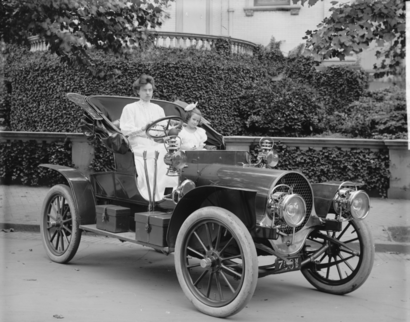
\includegraphics[width=\linewidth]{sample-franklin}
%   \caption{1907 Franklin Model D roadster. Photograph by Harris \&
%     Ewing, Inc. [Public domain], via Wikimedia
%     Commons. (\url{https://goo.gl/VLCRBB}).}
%   \Description{A woman and a girl in white dresses sit in an open car.}
% \end{figure}

% Your figures should contain a caption which describes the figure to
% the reader.

% Figure captions are placed {\itshape below} the figure.

% Every figure should also have a figure description unless it is purely
% decorative. These descriptions convey what’s in the image to someone
% who cannot see it. They are also used by search engine crawlers for
% indexing images, and when images cannot be loaded.

% A figure description must be unformatted plain text less than 2000
% characters long (including spaces).  {\bfseries Figure descriptions
%   should not repeat the figure caption – their purpose is to capture
%   important information that is not already provided in the caption or
%   the main text of the paper.} For figures that convey important and
% complex new information, a short text description may not be
% adequate. More complex alternative descriptions can be placed in an
% appendix and referenced in a short figure description. For example,
% provide a data table capturing the information in a bar chart, or a
% structured list representing a graph.  For additional information
% regarding how best to write figure descriptions and why doing this is
% so important, please see
% \url{https://www.acm.org/publications/taps/describing-figures/}.

%%
%% The next two lines define the bibliography style to be used, and
%% the bibliography file.
\bibliographystyle{ACM-Reference-Format}
\bibliography{sample-base}

\end{document}
\endinput
%%
%% End of file `sample-acmtog.tex'.
